\textbf{\hypertarget{P7}{[\,Suggested Time: 20 mins \textbar \, Total Marks: 10 \textbar \, Challenging\,]}}\\
%%%%%Question i, Proving the parallel eff. resistance equation%%%%%
\\
\textbf{Circuit Theory} \\
\textit{The workings of a parallel circuit can be explained with a water tank, where the water \\
        tank is like a battery in the circuit, current \(I\) is the water flowing in the pipes, \\
        voltage \(V\) can be seen as the pressure which the water experiences at a \\
        certain point and resistance \(R\) is a measure of how much pressure is \\
        needed to move a certain quantity of water from a point to another}
\begin{center}
    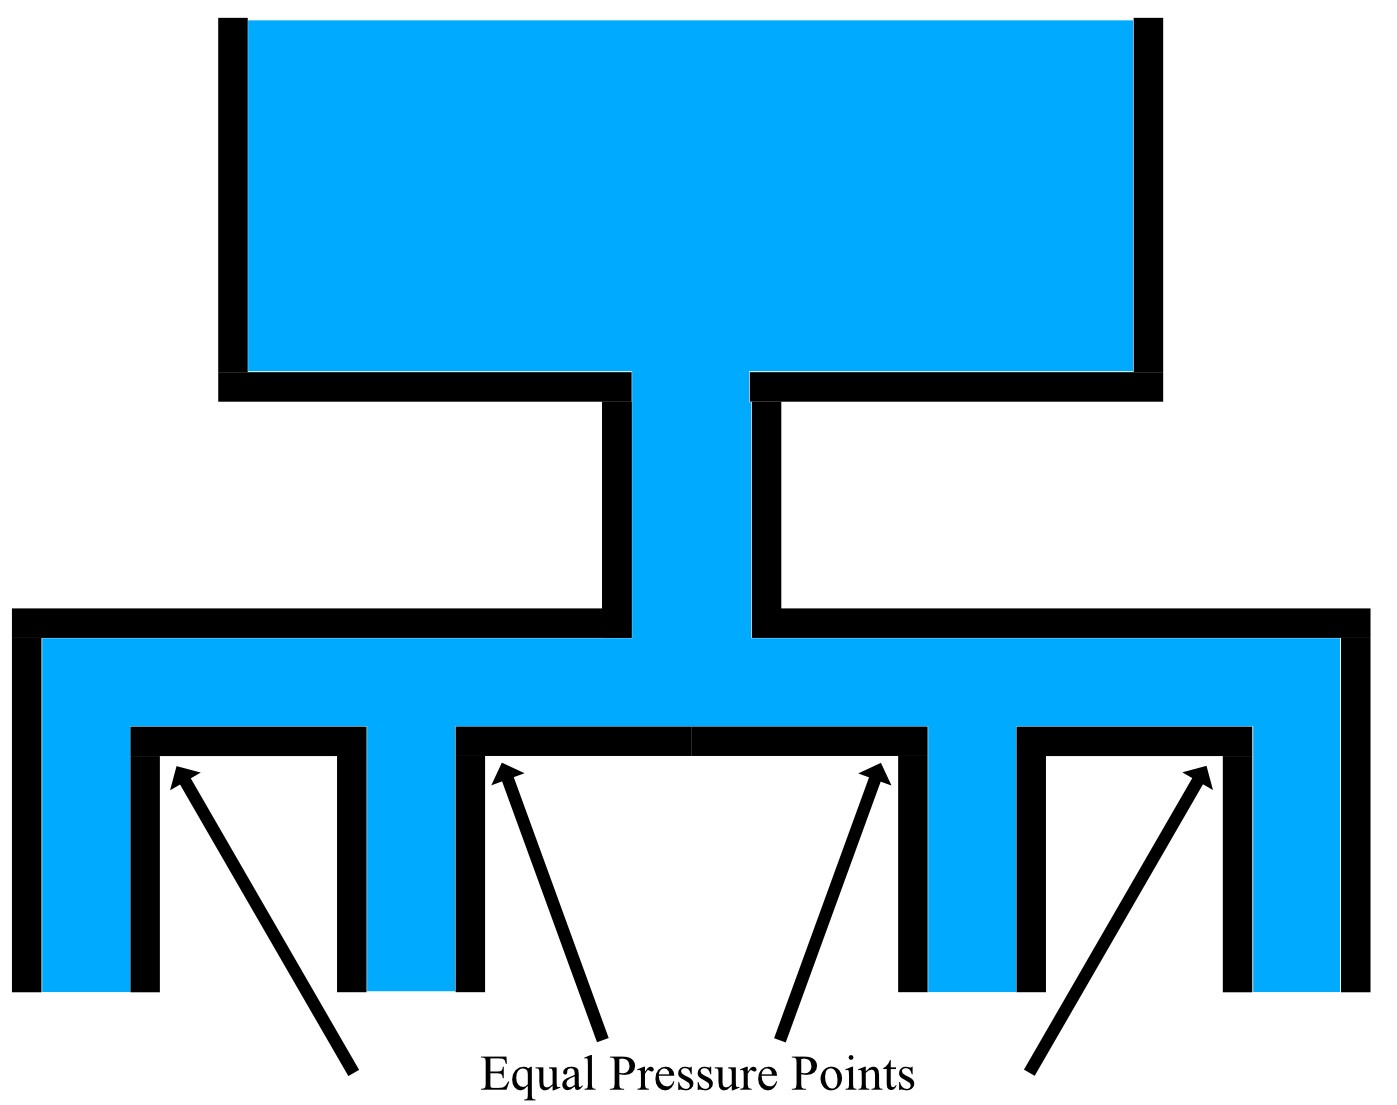
\includegraphics[scale=0.7]{Question 7i - Water Tank.jpg}
\end{center}
\textit{In the diagram shown above, it is known that the pressure at all 4 points which the arrows \\
        are pointing at are equivalent, and the total volume of water that flows out of the pipes \\
        is equal to the volume of water that flows into the  pipes from the water tank. \\
        \\
        It is also given that ohmic conductors follow ohm's law, \(V = IR\) \\
}

\begin{center}
    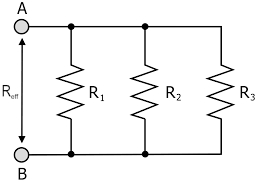
\includegraphics[scale=1.2]{Question 7i - Circuit Diagram.jpg}
\end{center}

\newpage

\textit{
    \textbf{(i)} Using the information given above, deduce the effective resistance, \(R_{eff}\), in \\
    \hspace*{20pt} the circuit shown above, and consequently, find an expression for a parallel \\
    \hspace*{20pt} circuit with n resistors. \textbf{Leave your answers in terms of V,I and R}
} \qnmark{5} \\

%%%%%%%%%%%%%%%%%%
%%%%%Solution%%%%%
%%%%%%%%%%%%%%%%%%

%\begin{comment}

%%%%%Electricity laws in a parallel circuit%%%%%
\textit{From the question, we can deduce that the
}
\begin{gather*}
    Total \; current, \; I_{T}, \; in \; the \; circuit \; is \; I_{T} = I_{1}+I_{2}+I_{3} \\
    Total \; voltage, \; V_{T}, \; across \; the \; circuit \; is \; V_{T} = V_{1} = V_{2} = V_{3} \onemark \\
\end{gather*}
\textit{By Ohm's law, we can see that}
\begin{equation*}
    \displaystyle I_{1} = \frac{V_{1}}{R_{1}}, I_{2} = \frac{V_{2}}{R_{2}}, I_{3} = \frac{V_{3}}{R_{3}} \onemark \\
\end{equation*}

%%%%%Proving R_{eff} for 3 resistors%%%%%
\textit{Using the total current and voltage equations that we had deduced,}
\begin{align*}
    \displaystyle I_{T} &= \frac{V_{1}}{R_{1}} + \frac{V_{2}}{R_{2}} + \frac{V_{3}}{R_{3}} \\
    \displaystyle       &= \frac{V_{T}}{R_{1}} + \frac{V_{T}}{R_{2}} + \frac{V_{T}}{R_{3}} \\
    \displaystyle       &= V_{T}\left(\frac{1}{R_{1}} + \frac{1}{R_{2}} + \frac{1}{R_{3}}\right) \onemark \\
\end{align*}
\begin{align*}
    \displaystyle \therefore R_{eff} &= \frac{V_{T}}{I_{T}} \\
    \displaystyle                    &= \frac{V_{T}}{V_{T}\left(\displaystyle \frac{1}{R_{1}} + \frac{1}{R_{2}} + \frac{1}{R_{3}}\right)} \\
    \displaystyle                    &= \frac{1}{\left(\displaystyle \frac{1}{R_{1}} + \frac{1}{R_{2}} + \frac{1}{R_{3}}\right)} \\
    \displaystyle                    &= \left(\displaystyle \frac{1}{R_{1}} + \frac{1}{R_{2}} + \frac{1}{R_{3}}\right)^{-1} \tag*{\qedsymbol} \\ \onemark \\
\end{align*}

%%%%%Proving the equation in the question%%%%%
\textit{Since we know that \(V_{T} = V_{1} = V_{2} = V_{3} = \cdots\), \\
        and that \(V_{T}\) would be eliminated in the expression, \\
        \\
        Following the same process, we can generalize the expression for n resistors as
}
\begin{gather*}
    \displaystyle R_{eff} = \left(\frac{1}{R_{1}}+\frac{1}{R_{2}}+\frac{1}{R_{3}}+\cdots+\frac{1}{R_{n}}\right)^{-1} \tag*{\qedsymbol} \\ \onemark
\end{gather*}

%\end{comment}

\newpage \ \newpage %Don't Comment

%%%%%Question iia, finding the eff. resistance of a parallel resistor system%%%%%
\begin{center}
    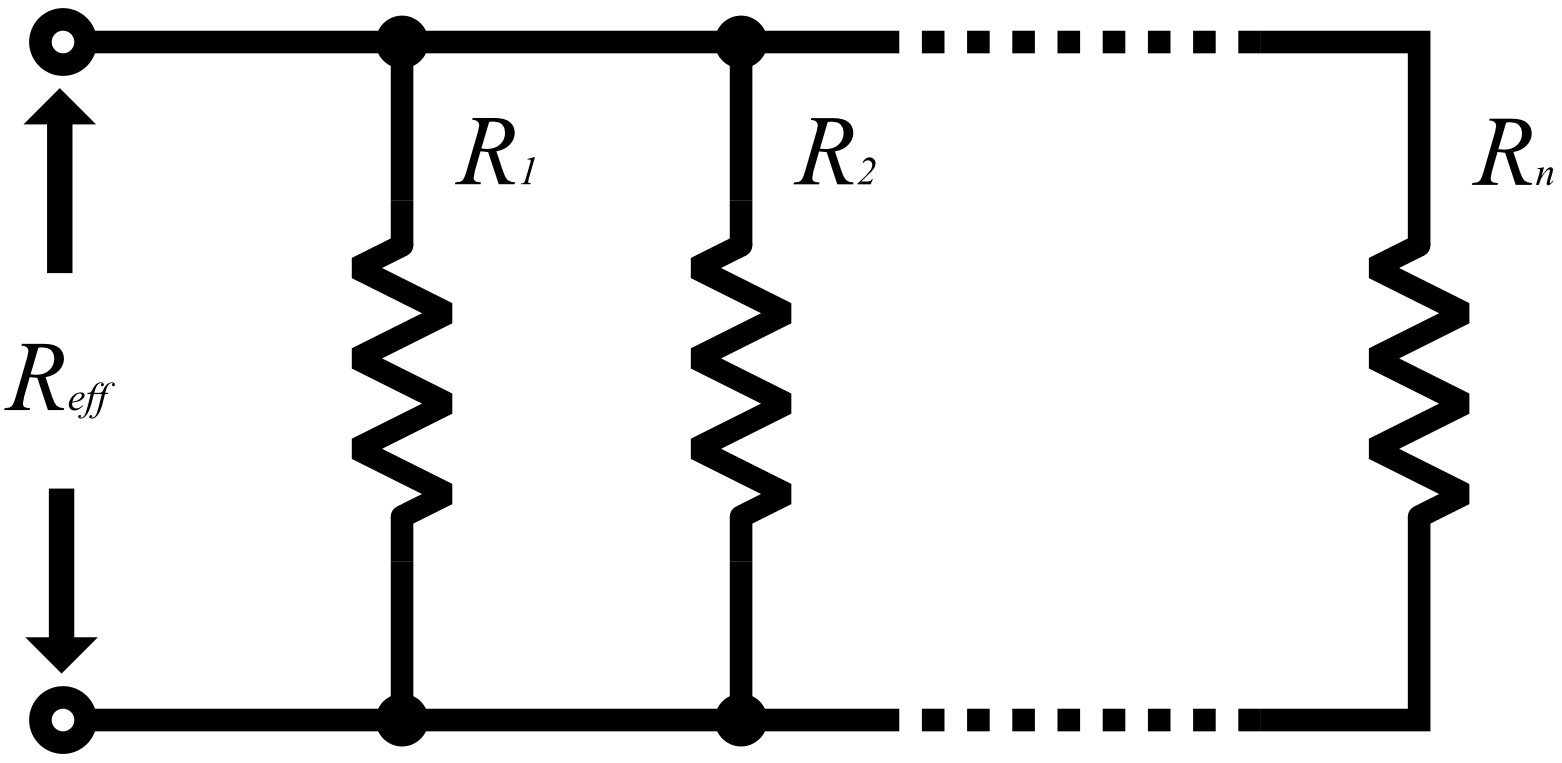
\includegraphics[scale=0.25]{Question 7iia - Circuit Diagram.jpg}
\end{center}
\textit{\textbf{(ii)(a)} Hence, using (i) or otherwise, find the effective resistance of the circuit shown above. \\
        \hspace*{35pt} Where \(R_{1} = \sqrt{1}+\sqrt{2}, R_{2} = \sqrt{2}+\sqrt{3}, R_{3} = \sqrt{3}+\sqrt{4} \; \cdots\) \\
        \hspace*{35pt} \textbf{Leave your answers in exact values}, and in terms of n.
} \qnmark{4} \\

%%%%%%%%%%%%%%%%%%
%%%%%Solution%%%%%
%%%%%%%%%%%%%%%%%%

%\begin{comment}

%%%%%Finding the effective resistance%%%%%
\textit{We can see that the resistance of the resistors follow a series with a general term of}
\begin{equation*}
    \displaystyle R_{n} = \sqrt{n}+\sqrt{n+1} \onemark \\
\end{equation*}

\begin{align*}
    \displaystyle \therefore R_{eff} &= \left(\frac{1}{\sqrt{1}+\sqrt{2}}+\frac{1}{\sqrt{2}+\sqrt{3}}+\frac{1}{\sqrt{3}+\sqrt{4}}+\cdots+\frac{1}{\sqrt{n}+\sqrt{n+1}}\right)^{-1} \onemark \\
    \displaystyle                    &= \left(\frac{\sqrt{1}-\sqrt{2}}{1-2}+\frac{\sqrt{2}-\sqrt{3}}{2-3}+\frac{\sqrt{3}-\sqrt{4}}{3-4}+\cdots+\frac{\sqrt{n}-\sqrt{n+1}}{n-n-1}\right)^{-1} \onemark \\
    \displaystyle                    &= \left(\left(\sqrt{2}-\sqrt{1}\right)+\left(\sqrt{3}-\sqrt{2}\right)+\left(\sqrt{4}-\sqrt{3}\right)+\cdots+\left(\sqrt{n+1}-\sqrt{n}\right)\right)^{-1} \\
    \displaystyle                    &= \left(\sqrt{n+1}-1\right)^{-1} \\
    \displaystyle                    &= \frac{1}{\sqrt{n+1}-1} \onemark
\end{align*}

\textit{The effective resistance of the circuit is \(\displaystyle \frac{1}{\sqrt{n+1}-1}\), \\ \
        where n is the number of resistors
}

%\end{comment}

\newpage \ \newpage %Don't Comment

%%%%%Question iib, proving if this is converging series%%%%%
\textit{\textbf{(ii)(b)} Explain, with relevant workings, if the effective resistance of the circuit \\
        \hspace*{40pt} will approach a unique value as more resistors are added into the circuit.
} \qnmark{1} \\

%%%%%%%%%%%%%%%%%%
%%%%%Solution%%%%%
%%%%%%%%%%%%%%%%%%

%\begin{comment}

\textit{from (ii)(a), \(\displaystyle R_{eff} = \frac{1}{\sqrt{n+1}-1}\)} \\
\begin{align*}
    \displaystyle As \; n \rightarrow \infty, \; \sqrt{n+1}-1 &\rightarrow \infty \\
    \displaystyle                      \frac{1}{\sqrt{n+1}-1} &\rightarrow 0 \\
    \displaystyle                          \therefore R_{eff} &\rightarrow 0 \onemark
\end{align*}
\textit{Yes, \(R_{eff}\) approaches the value 0 as more resistors are added into the circuit}


%\end{comment}